\documentclass[11pt]{article}

% Language setting 
\usepackage[spanish]{babel}

% Set page size and margins
\usepackage[a4paper,top=2cm,bottom=2cm,left=3cm,right=3cm,marginparwidth=1.75cm]{geometry}
\setlength
\parindent{0pt}

% Useful packages 
\usepackage{amsmath} 
\usepackage{graphicx}
\usepackage[colorlinks=true, linkcolor=black, urlcolor=blue]{hyperref}

% Uncomment these packages if you want to use dark mode % \usepackage{darkmode}
% \enabledarkmode

\usepackage{listings}
\usepackage{tcolorbox}
\usepackage{blindtext}  % For dummy text

\lstset{
    keywordstyle=\color{blue}\bfseries,
    basicstyle=\ttfamily\fontsize{10pt}{\baselineskip}\selectfont,
}



% Title and author 
\title{Tarea: Automatización de Software en el entorno MVF}
\author{Álvaro Hernández} 
\date{\today}

\begin{document}

%%%%%%%%%%%%%%%%%%%%%%%%%%%%%%%%%%

\maketitle 
\tableofcontents 
\newpage

\section*{Introducción}

En este trabajo se realizará una automatización de la configuración de una red de routers Cisco que se proporciona en el enuciado.
Para ello, se utilizará el software GNS3 para inizialicar y simular la red, y a ésta se aplicarán técnicas y configuraciones de automatización, monitorización, y gestión de red. 
El software que se usará para las distintas tareas será:

\begin{itemize}
    \item \textbf{Simulación}: Para la simulación, como se ha comentado antes, se usará GNS3 a partir de la topología proporcionada.
    \item \textbf{Automatización}: Aunque se haya mencionado el posible uso de scripts de Python en el enunciado, se usará Ansible para todas las tareas de automatización posibles, se intentará mantener todo en el mismo \textbf{archivo yaml}
    \item \textbf{Monitorización}: Se usará el \textbf{protocolo SNMP} para la monitorización de la red, con software como Cacti, OpenObserver o MIB Browser.
\end{itemize}

\section{Implementación / Configuración de la topología}

El primer ejercicio trata sobre la implementación de la topología proporcionada por el mismo. Se realiza el diseño mediante GNS3, sin configurar nada más que añadir las conexiones de todos los elementos. Tras esto, la topología queda de la siguiente manera:


\begin{figure}[h]
    \centering
    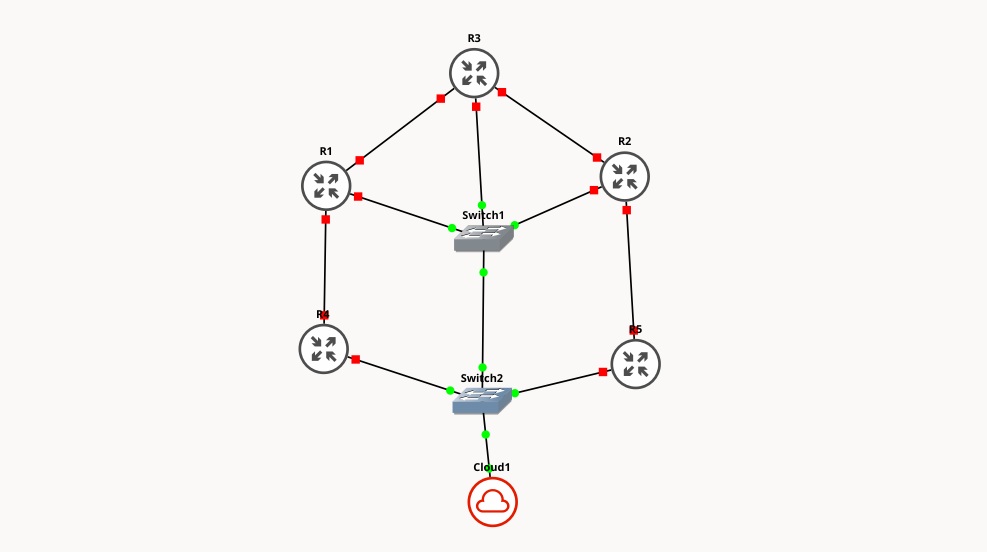
\includegraphics[width=\textwidth]{src/topologia.png}
    \caption{Topología de la red}
\end{figure}

No se ha configurado ni hostnames ni interfaces para dejarle el trabajo a Ansible.

Para iniciar con la configuración, que se hará mediante Ansible, hará falta configurar ssh para la conexión de forma segura, y una ip de interfaz para poder realizar la conexión. Por lo que mediante GNS3 se configurará lo mínimo necesario para este funcionamiento. Esta configuración será la proporcionada en \href{https://github.com/plopezmp/GdR}{el Github de configuración de Ansible de la asignatura}, adaptando las IPs e interfaces a nuestra topología. Un ejemplo con el MU-NN sería el siguiente (desde la configuración del router ya):

\begin{tcolorbox}[
    boxrule=0pt,
]
    \begin{lstlisting}[gobble=6]
        int g0/0 
        ip address 172.18.0.220 255.255.255.0
        exit
        line vty 0 15
        login local
        transport input all
        exit 
        enable secret cisco 
        line console 0 
        passw cisco
        login 
        exit 
        ip domain-name upct 
        username ansible privilege 15 secret ansible
        ip ssh time-out 60
        crypto key generate rsa usage-keys label router-key
        # Y seleccionamos 1024 bits para ambas opciones.
    \end{lstlisting}
\end{tcolorbox}

Con esto se podría realizar la conexión con ssh, por lo que Ansible se podrá conectar. Comprobamos que se puede conectar a ssh con el usuario ansible y la contraseña ansible.

\begin{figure}[h]
    \centering
    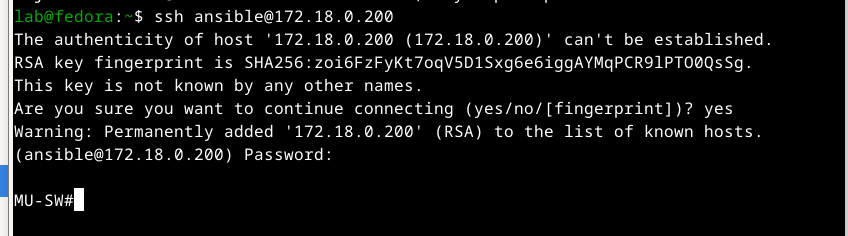
\includegraphics[width=\textwidth]{src/ssh.png}
    \caption{Conexión ssh con el router MU-Sw}
\end{figure}

Una vez comprobado que todos los routers se pueden conectar mediante ssh, se procede a la configuración de Ansible. Se pide configurar el resto de las interfaces junto al loopback y hostnames. 

Para iniciar con la configuración, se creará un archivo \texttt{hosts} con los routers que se quieren configurar, y se reciclará el archivo \texttt{ansible.cfg} del repositorio de la asignatura para que Ansible no pida confirmación para las conexiones ssh. El archivo hosts está accesible en la entrega del trabajo. 

Para las \textbf{plays} de Ansible, se ha creado un archivo \texttt{tarea.yml} que recoge todas las acciones que hará ansible en un único archivo. Cada router tendrá una play, por lo que nuestra \texttt{tarea.yml} tendrá este formato:

\begin{tcolorbox}[
    boxrule=0pt,
    title=Formato que seguirá tarea.yml,
]
    \begin{lstlisting}[gobble=6]
        --- - name: Configure interface g1/0 on the router 
        hosts: R1
        gather\_facts: no 
        connection: network\_cli 
        tasks:
            - name: Configure router...
            ios\_command:
                commands:
                    - interface GigabitEthernet1/0
                    - ... 
                register: output

    \end{lstlisting}
\end{tcolorbox}

Una vez terminado el archivo \texttt{tarea.yml}, donde cada router tendrá la configuración de sus interfaces respectivas, se ejecutará de la siguiente forma para que se realicen las configuraciones:

\begin{tcolorbox}[
    boxrule=0pt,
    title=Script de ejecución de Ansible,
]
    \begin{lstlisting}[language=bash, gobble=6]
        #! /bin/bash

        workon ansible
        ansible-playbook -i hosts tarea.yml
        #-i para indicar los inputs que seran hosts y tarea.yml
    \end{lstlisting}
\end{tcolorbox}

Si la ejecución es correcta, tendremos el siguiente output de Ansible que nos indica que no han habido errores:

\begin{figure}[h]
    \centering
    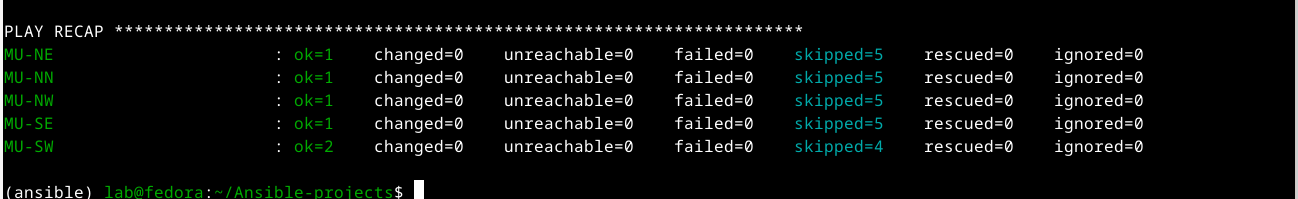
\includegraphics[width=\textwidth]{src/ansible.png}
    \caption{Output de Ansible tras la ejecución}
\end{figure}

\section{Encaminamiento}

\section{Activación de la gestión SNMP de los routers}
\section{Configuraciónd de Alarmas}
\section{Generación de tráfico Cisco IP SLA}
\section{Monitorización con Cacti}
\section{Monitorización de flujos de tráfico}

\end{document}